\documentclass[11pt]{article}
\usepackage[textwidth=18.0cm, textheight=23.0cm, top=2.0cm]{geometry}
\usepackage{pst-all}
\usepackage{amssymb}
\usepackage{tikz}
\usepackage{underscore}\begin{document}
\pagestyle{empty}


ClassName: \underline{\textbf{Class_06.2bp-11}}
\par
BinSize: \underline{\textbf{300 × 300}}
\par
ReduceSize: \underline{\textbf{300 × 300}}
\par
TypeNum: \underline{\textbf{40}}
\par
Num: \underline{\textbf{40}}
\par
OutS: \underline{\textbf{180000}}
\par
InS: \underline{\textbf{89131}}
\par
Rate: \underline{\textbf{0.495}}
\par
UB: \underline{\textbf{2}}
\par
LB0: \underline{\textbf{1}}
\par
LB: \underline{\textbf{2}}
\par
LBWithCut: \underline{\textbf{2}}
\par
NodeCut: \underline{\textbf{0}}
\par
ExtendedNodeCnt: \underline{\textbf{1}}
\par
GenNodeCnt: \underline{\textbf{1}}
\par
PrimalNode: \underline{\textbf{0}}
\par
ColumnCount: \underline{\textbf{72}}
\par
TotalCutCount: \underline{\textbf{0}}
\par
RootCutCount: \underline{\textbf{0}}
\par
LPSolverCnt: \underline{\textbf{71}}
\par
PricingSolverCnt: \underline{\textbf{71}}
\par
BranchAndBoundNum: \underline{\textbf{1}}
\par
isOpt: \underline{\textbf{false}}
\par
TimeOnInitSolution: \underline{\textbf{600.000 s}}
\par
TimeOnPrimal: \underline{\textbf{0.000 s}}
\par
TimeOnPricing: \underline{\textbf{2999.687 s}}
\par
TimeOnRmp: \underline{\textbf{0.085 s}}
\par
TotalTime: \underline{\textbf{3600.006 s}}
\par
\newpage


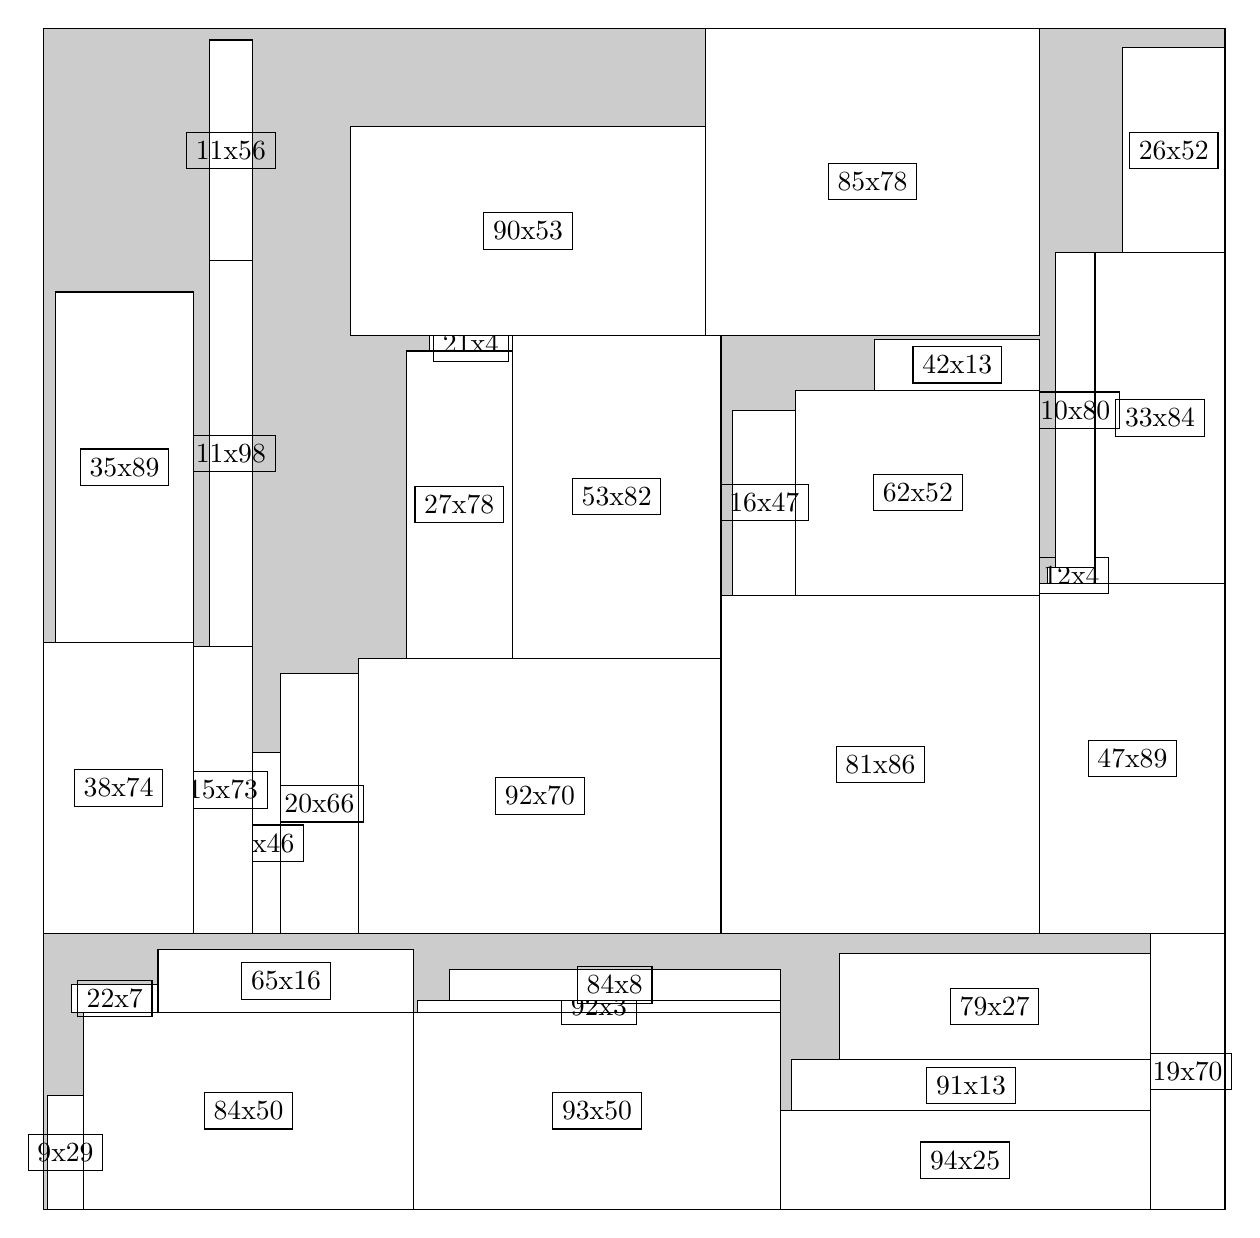
\begin{tikzpicture}[shorten >=1pt,scale=1.0,every node/.style={scale=1.0},->]
\tikzstyle{vertex}=[circle,fill=black!25,minimum size=14pt,inner sep=0pt]
\filldraw[fill=gray!40!white, draw=black] (0,0) rectangle (15.0,15.0);
\foreach \name/\x/\y/\w/\h in {19x70/14.05/0.0/0.9500000000000001/3.5,94x25/9.35/0.0/4.7/1.25,91x13/9.5/1.25/4.55/0.65,79x27/10.100000000000001/1.9000000000000001/3.95/1.35,93x50/4.7/0.0/4.65/2.5,92x3/4.75/2.5/4.6000000000000005/0.15000000000000002,84x8/5.15/2.6500000000000004/4.2/0.4,84x50/0.5/0.0/4.2/2.5,9x29/0.05/0.0/0.45/1.4500000000000002,65x16/1.4500000000000002/2.5/3.25/0.8,22x7/0.35000000000000003/2.5/1.1/0.35000000000000003,47x89/12.65/3.5/2.35/4.45,33x84/13.350000000000001/7.95/1.6500000000000001/4.2,12x4/12.75/7.95/0.6000000000000001/0.2,10x80/12.850000000000001/8.15/0.5/4.0,26x52/13.700000000000001/12.15/1.3/2.6,81x86/8.6/3.5/4.05/4.3,62x52/9.55/7.800000000000001/3.1/2.6,42x13/10.55/10.4/2.1/0.65,16x47/8.75/7.800000000000001/0.8/2.35,92x70/4.0/3.5/4.6000000000000005/3.5,20x66/3.0/3.5/1.0/3.3000000000000003,7x46/2.6500000000000004/3.5/0.35000000000000003/2.3000000000000003,53x82/5.95/7.0/2.6500000000000004/4.1000000000000005,27x78/4.6000000000000005/7.0/1.35/3.9000000000000004,21x4/4.9/10.9/1.05/0.2,85x78/8.4/11.100000000000001/4.25/3.9000000000000004,90x53/3.9000000000000004/11.100000000000001/4.5/2.6500000000000004,15x73/1.9000000000000001/3.5/0.75/3.6500000000000004,11x98/2.1/7.15/0.55/4.9,11x56/2.1/12.05/0.55/2.8000000000000003,38x74/0.0/3.5/1.9000000000000001/3.7,35x89/0.15000000000000002/7.2/1.75/4.45}
\filldraw[fill=white!40!white, draw=black] (\x,\y) rectangle node[draw] (\name) {\name} ++(\w,\h);
\end{tikzpicture}


w =19 , h =70 , x =281 , y =0 , v =1330
\par
w =94 , h =25 , x =187 , y =0 , v =2350
\par
w =91 , h =13 , x =190 , y =25 , v =1183
\par
w =79 , h =27 , x =202 , y =38 , v =2133
\par
w =93 , h =50 , x =94 , y =0 , v =4650
\par
w =92 , h =3 , x =95 , y =50 , v =276
\par
w =84 , h =8 , x =103 , y =53 , v =672
\par
w =84 , h =50 , x =10 , y =0 , v =4200
\par
w =9 , h =29 , x =1 , y =0 , v =261
\par
w =65 , h =16 , x =29 , y =50 , v =1040
\par
w =22 , h =7 , x =7 , y =50 , v =154
\par
w =47 , h =89 , x =253 , y =70 , v =4183
\par
w =33 , h =84 , x =267 , y =159 , v =2772
\par
w =12 , h =4 , x =255 , y =159 , v =48
\par
w =10 , h =80 , x =257 , y =163 , v =800
\par
w =26 , h =52 , x =274 , y =243 , v =1352
\par
w =81 , h =86 , x =172 , y =70 , v =6966
\par
w =62 , h =52 , x =191 , y =156 , v =3224
\par
w =42 , h =13 , x =211 , y =208 , v =546
\par
w =16 , h =47 , x =175 , y =156 , v =752
\par
w =92 , h =70 , x =80 , y =70 , v =6440
\par
w =20 , h =66 , x =60 , y =70 , v =1320
\par
w =7 , h =46 , x =53 , y =70 , v =322
\par
w =53 , h =82 , x =119 , y =140 , v =4346
\par
w =27 , h =78 , x =92 , y =140 , v =2106
\par
w =21 , h =4 , x =98 , y =218 , v =84
\par
w =85 , h =78 , x =168 , y =222 , v =6630
\par
w =90 , h =53 , x =78 , y =222 , v =4770
\par
w =15 , h =73 , x =38 , y =70 , v =1095
\par
w =11 , h =98 , x =42 , y =143 , v =1078
\par
w =11 , h =56 , x =42 , y =241 , v =616
\par
w =38 , h =74 , x =0 , y =70 , v =2812
\par
w =35 , h =89 , x =3 , y =144 , v =3115
\par
\newpage


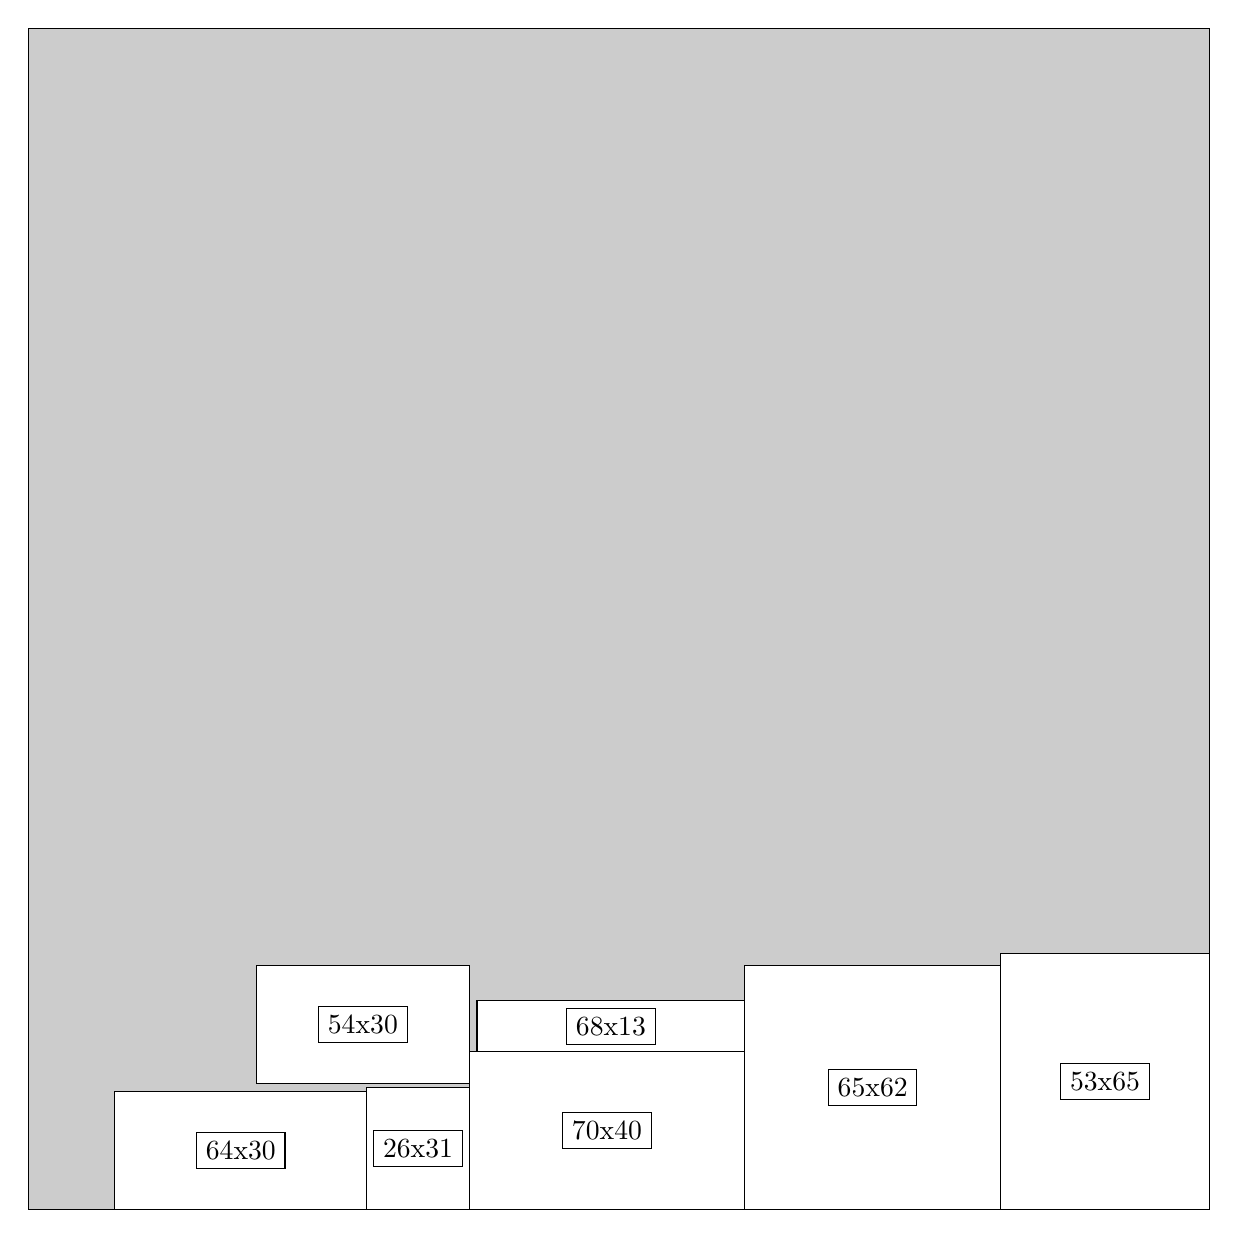
\begin{tikzpicture}[shorten >=1pt,scale=1.0,every node/.style={scale=1.0},->]
\tikzstyle{vertex}=[circle,fill=black!25,minimum size=14pt,inner sep=0pt]
\filldraw[fill=gray!40!white, draw=black] (0,0) rectangle (15.0,15.0);
\foreach \name/\x/\y/\w/\h in {53x65/12.350000000000001/0.0/2.6500000000000004/3.25,65x62/9.1/0.0/3.25/3.1,70x40/5.6000000000000005/0.0/3.5/2.0,68x13/5.7/2.0/3.4000000000000004/0.65,26x31/4.3/0.0/1.3/1.55,64x30/1.1/0.0/3.2/1.5,54x30/2.9000000000000004/1.6/2.7/1.5}
\filldraw[fill=white!40!white, draw=black] (\x,\y) rectangle node[draw] (\name) {\name} ++(\w,\h);
\end{tikzpicture}


w =53 , h =65 , x =247 , y =0 , v =3445
\par
w =65 , h =62 , x =182 , y =0 , v =4030
\par
w =70 , h =40 , x =112 , y =0 , v =2800
\par
w =68 , h =13 , x =114 , y =40 , v =884
\par
w =26 , h =31 , x =86 , y =0 , v =806
\par
w =64 , h =30 , x =22 , y =0 , v =1920
\par
w =54 , h =30 , x =58 , y =32 , v =1620
\par
\newpage


\end{document}